\documentclass[a4paper, 12pt]{article}
\usepackage[english,russian]{babel}
\usepackage{amsfonts}
\usepackage{graphicx}

\begin{document}
	\begin{Huge}
		\begin{center}
			\textbf{Отчет о выполнении лабораторной работы 1.1.1}\\
			\vspace{2em}
			\textbf{Определение систематических и случайных погрешностей при измерении удельного сопротивления нихромовой проволоки}\\
			\vspace{5em}
			\textbf{Выполнил: }Тимонин Андрей\\
			\textbf{Группа: }Б01-208\\
			\vspace{6em}
			\textbf{Дата: }15.09.2022\\
		\end{center}
	\end{Huge}
\textbf{1)Аннотация}\\
\textbf{Цель: }
измерить удельное сопротивление проволоки и вычислить систематические и случайные погрешности при использовании таких измерительных приборов, как линейка, штангенциркуль, микрометр, амперметр, вольтметр и мост постоянного тока. 
\vspace{1em}\\\textbf{Приборы: }
линейка, штангенциркуль, микрометр, отрезок проволоки из нихрома, амперметр, вольтметр, источник ЭДС, мост постоянного тока, реостат, ключ.\\ 
\vspace{1em}\\\textbf{Ожидаемые результаты:}
полученные результаты измерения удельного сопротивления проволоки совпадают с табличными значениями.\vspace{2em}
\vspace{2em}\textbf{2)Теоретические сведения}\\
\vspace{2em}\textbf{3)Методика измерений}\\
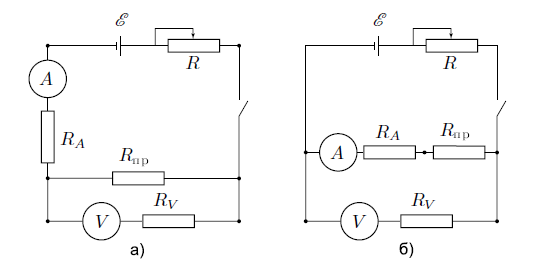
\includegraphics{1.png}\\
\vspace{2em}\textbf{4)Используемое оборудование}\\
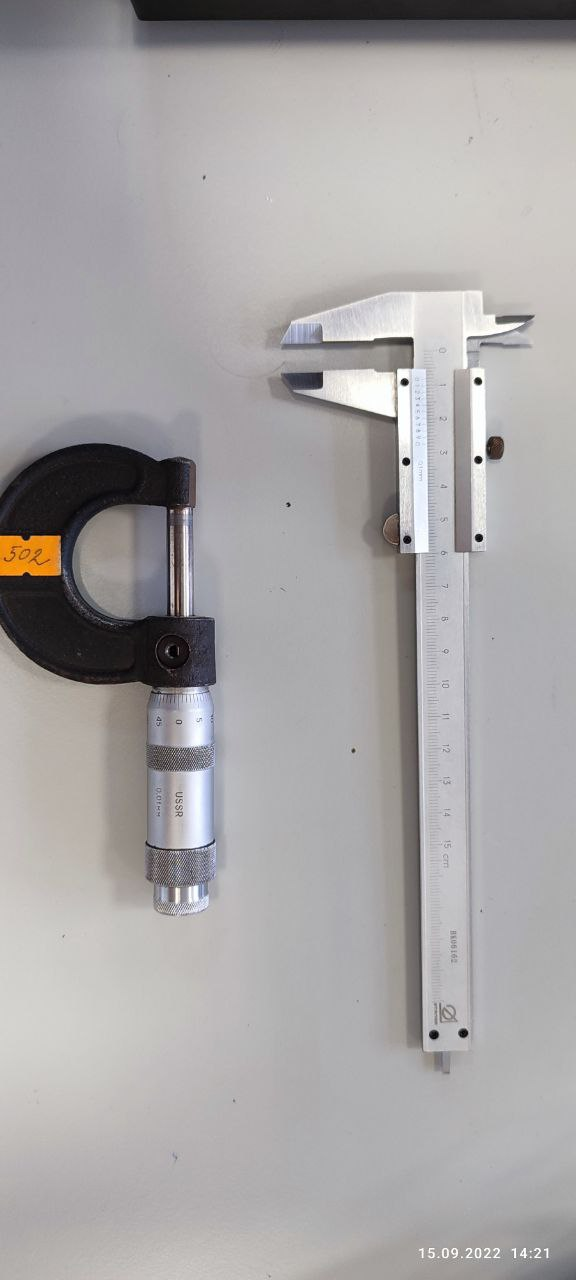
\includegraphics[width=10cm]{A (2).jpg}\\
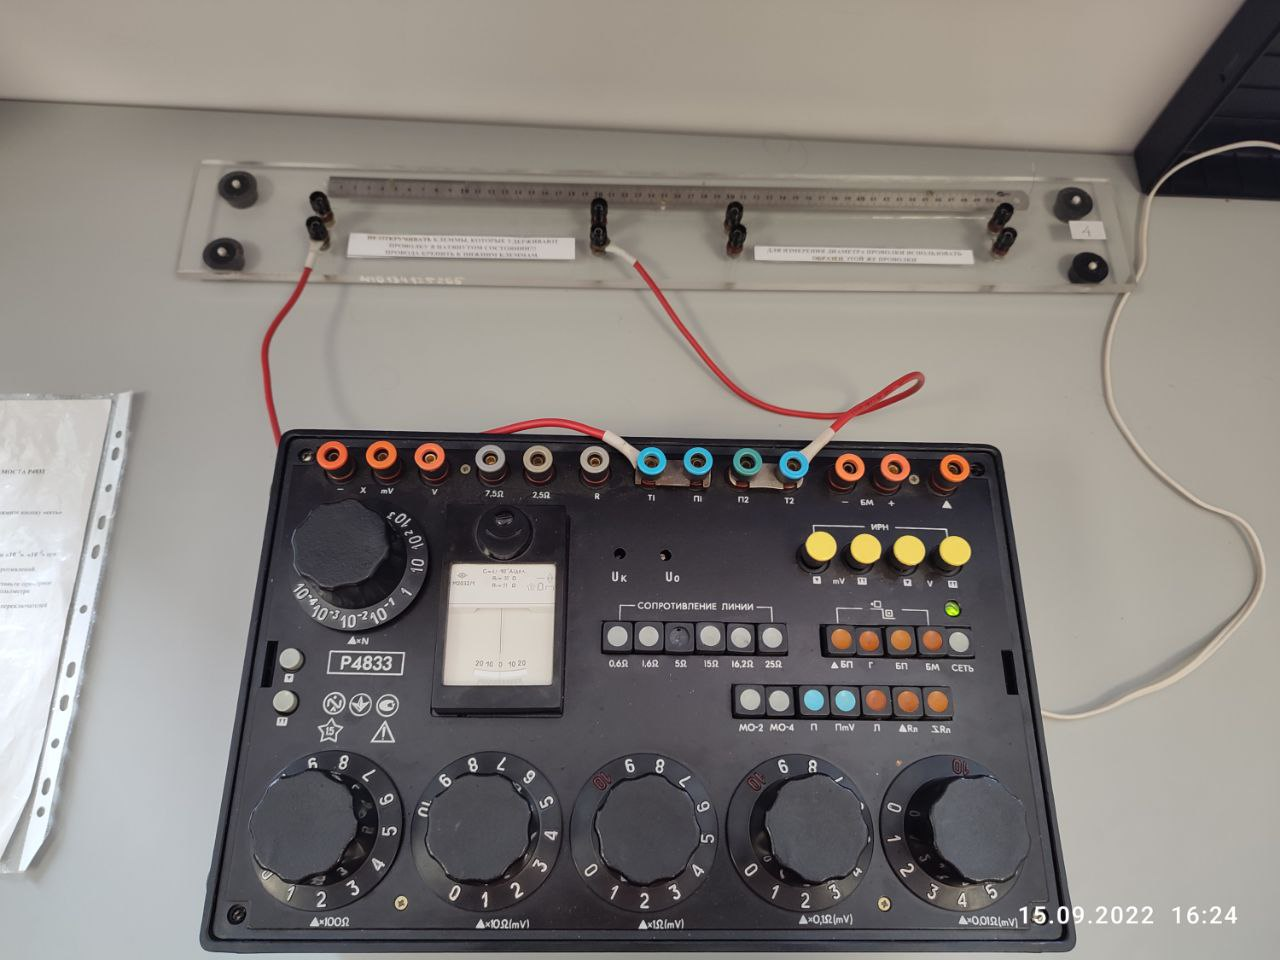
\includegraphics[width=13cm]{A (1).jpg}\\
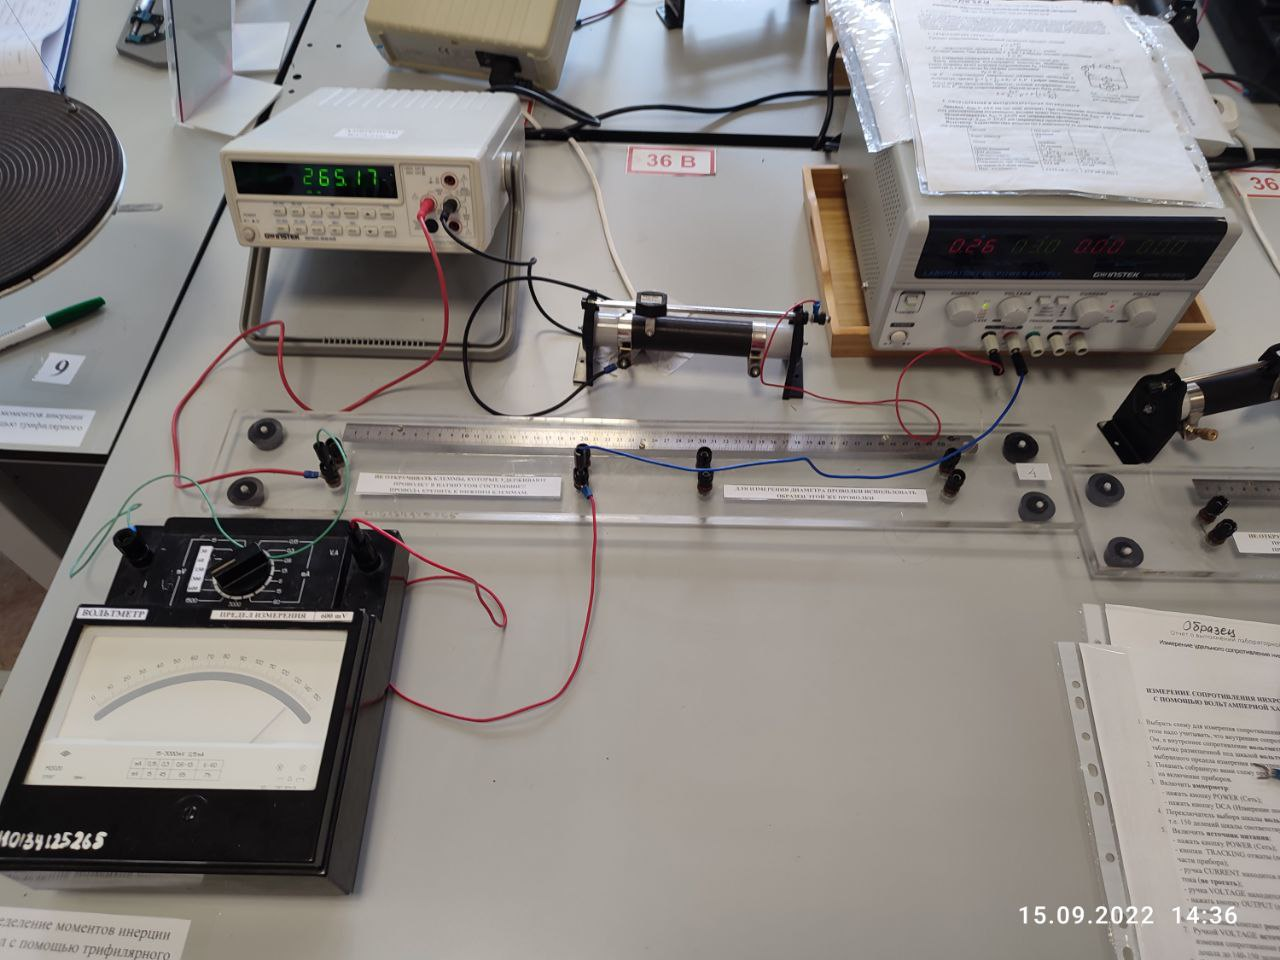
\includegraphics[width=13cm]{A (3).jpg}\\
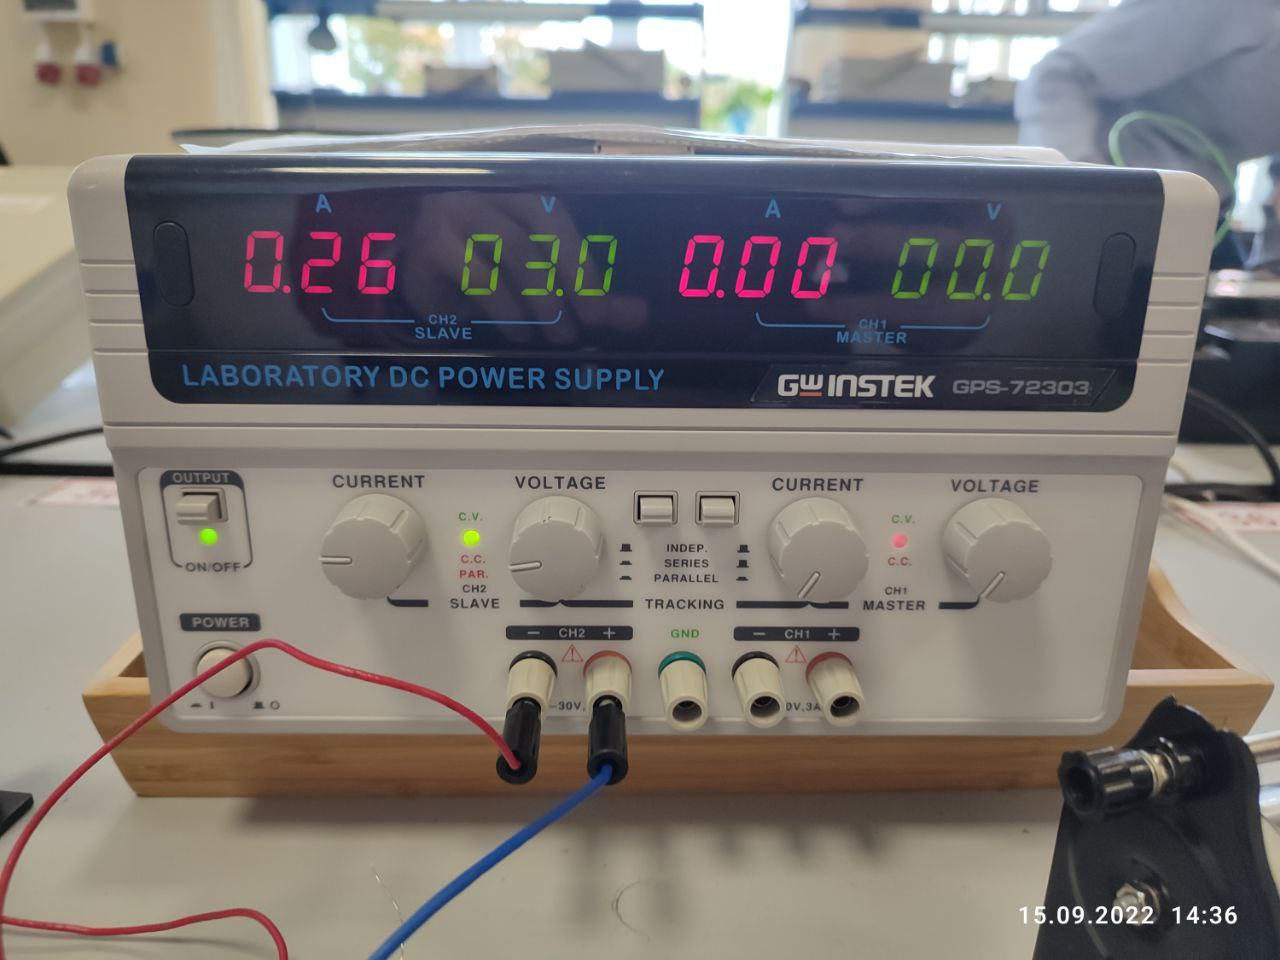
\includegraphics[width=13cm]{A (4).jpg}\\
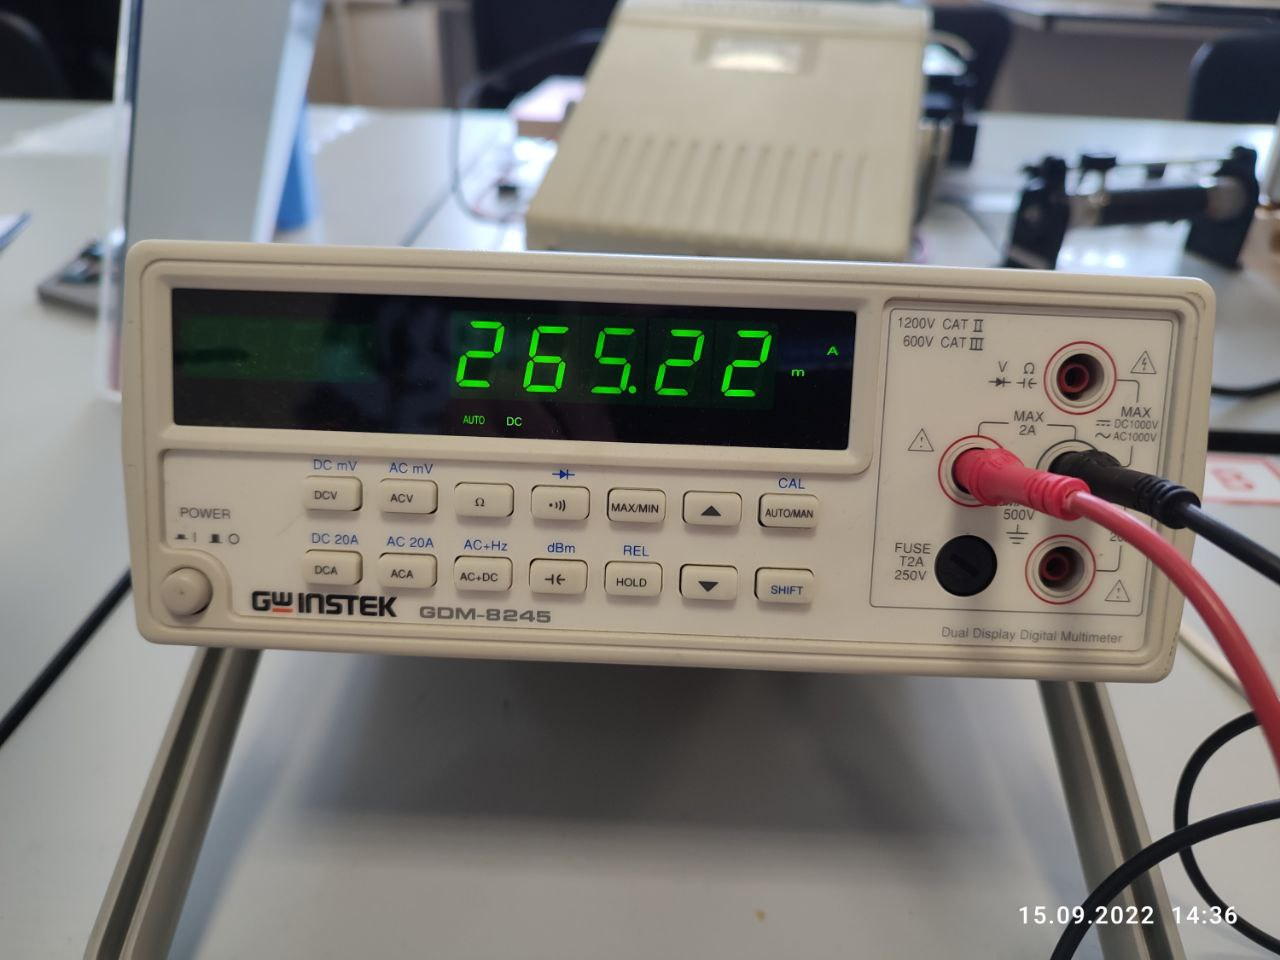
\includegraphics[width=13cm]{A (5).jpg}\\
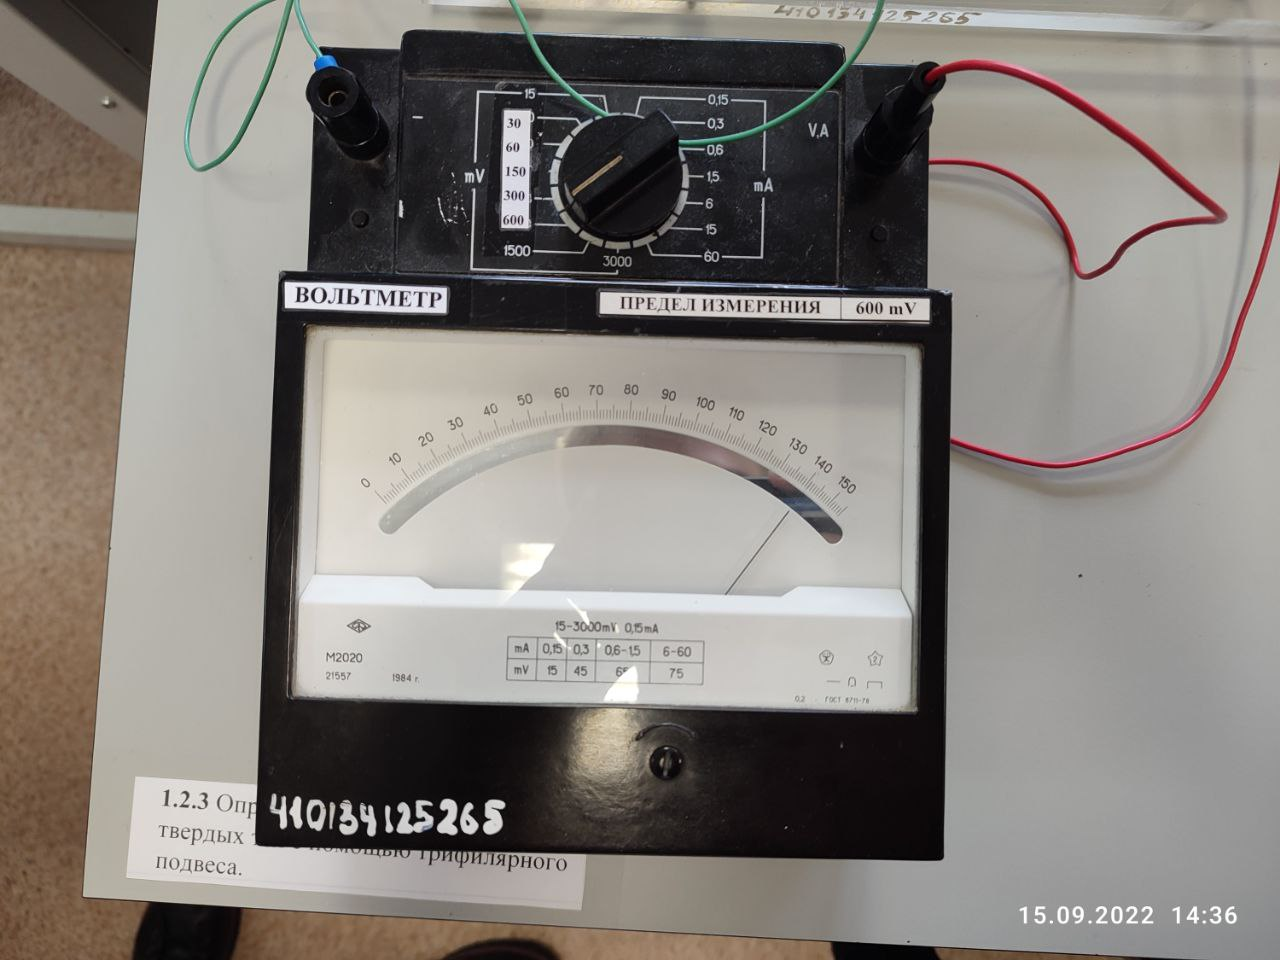
\includegraphics[width=13cm]{A (6).jpg}\\
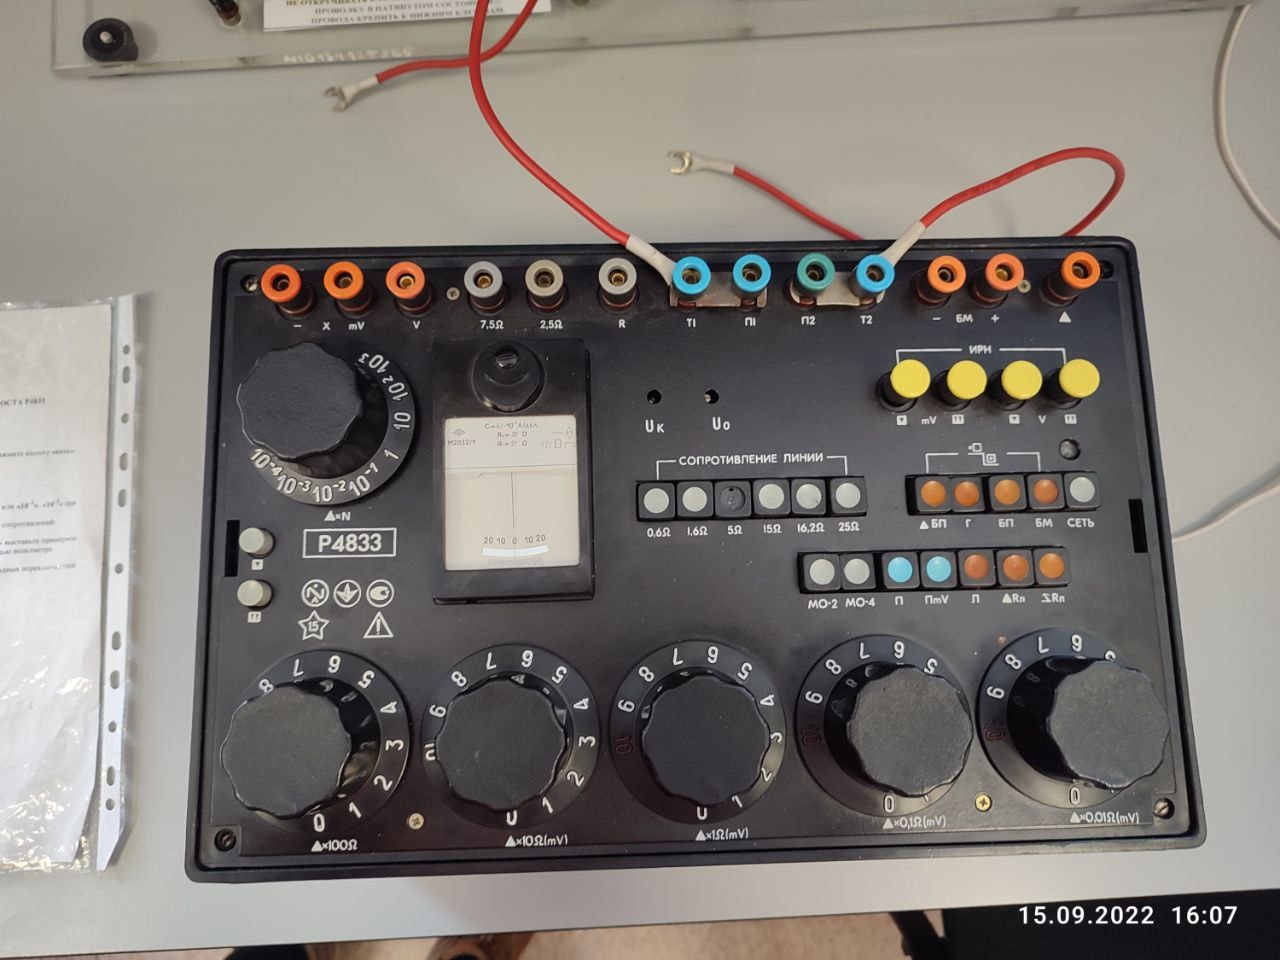
\includegraphics[width=13cm]{A (7).jpg}\\
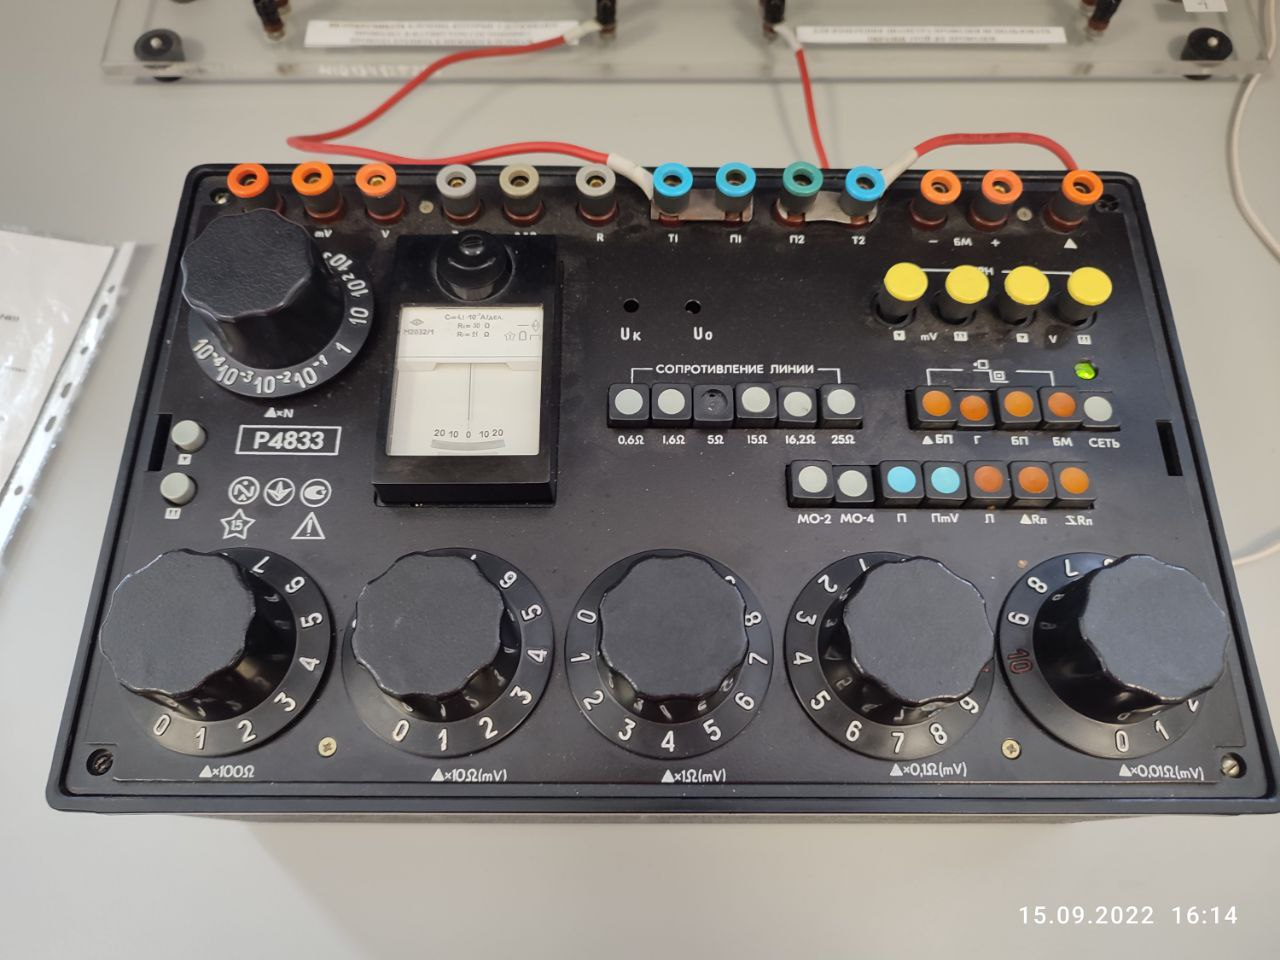
\includegraphics[width=13cm]{A (8).jpg}\\
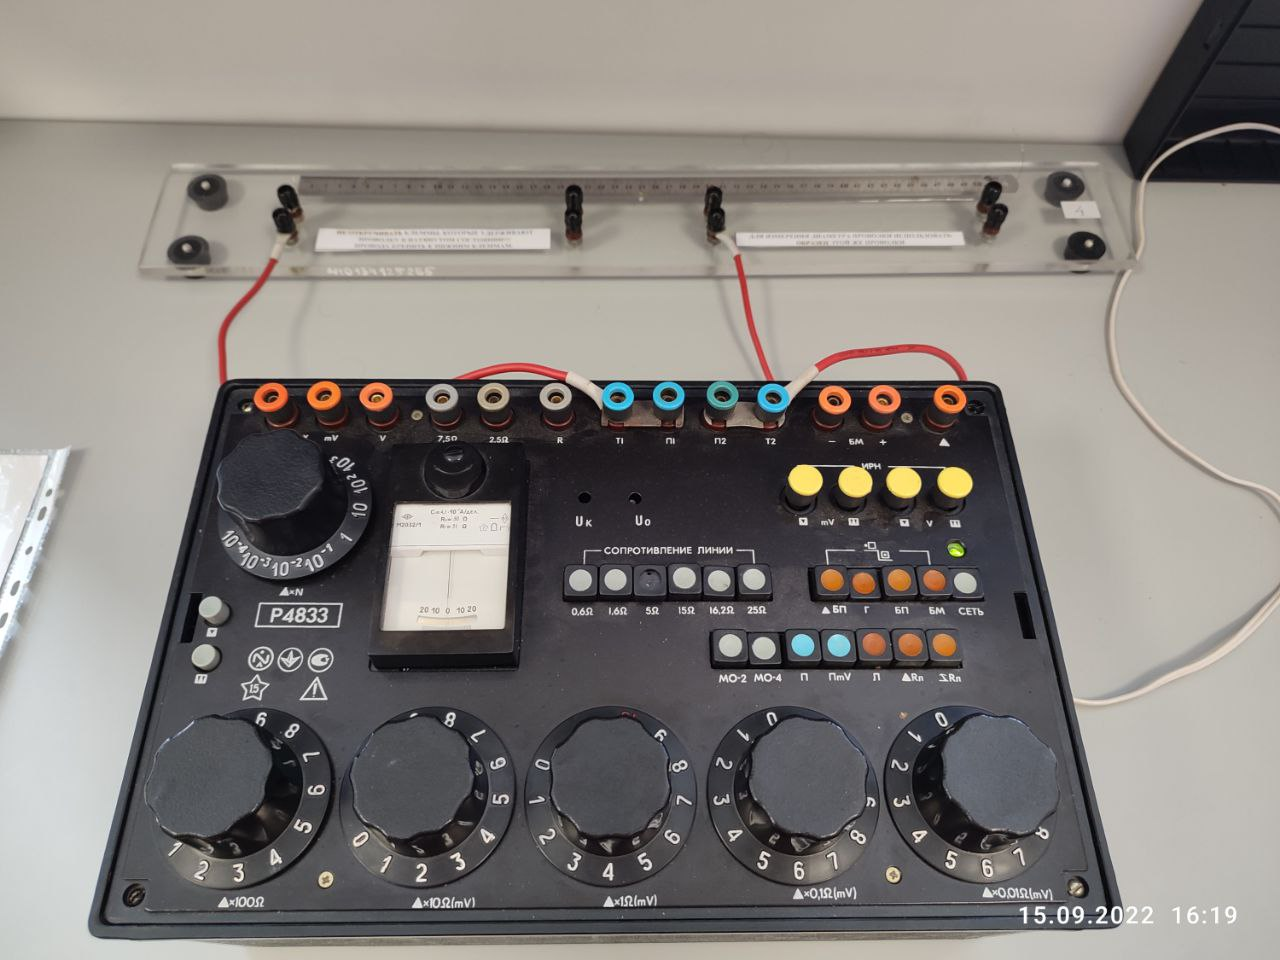
\includegraphics[width=13cm]{A (9).jpg}\\
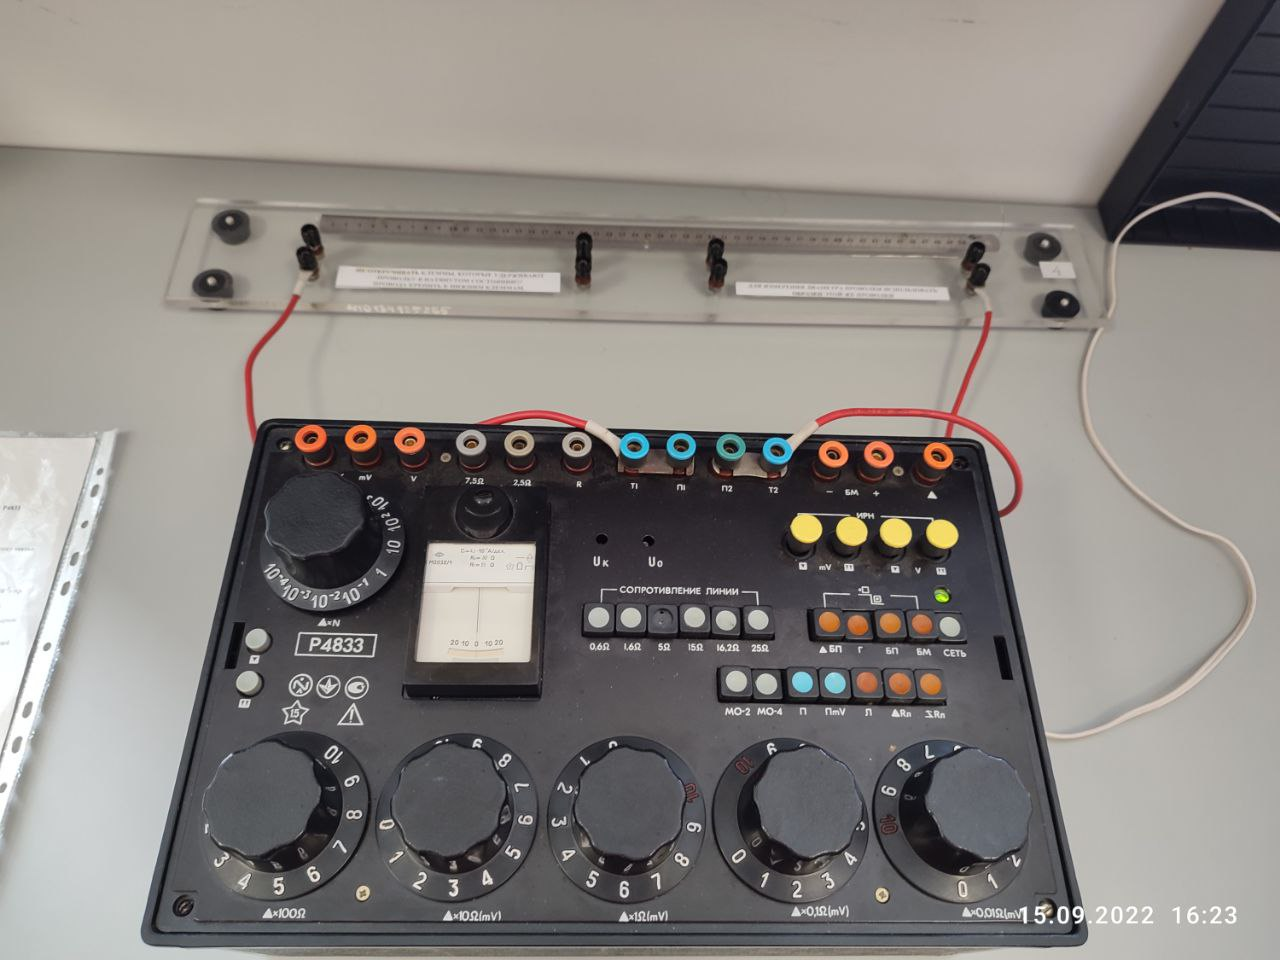
\includegraphics[width=13cm]{A (10).jpg}\\

\vspace{2em}\textbf{5)Результаты измерений и обработка данных}\\
\begin{center}
	\textbf{Показания амперметра и вольтметра}
\end{center}

\begin{center}
	\begin{tabular}{|c|c|c||c|c|c||c|c|c|}
		\hline
		\multicolumn{3}{ | c ||}{l = 20 см } & \multicolumn{3}{ | c ||}{l = 30 см } & \multicolumn{3}{ | c |}{l = 50 см }\\
		\hline
		U, мВ & $I, \frac{2мА}{дел}$  & I, мА & U, мВ & $I, \frac{2мА}{дел}$  & I, мА & U, мВ & $I, \frac{2мА}{дел}$  & I, мА \\
		\hline 
		201&49&88&279&45&90&478&46&92\\
		\hline 
		580.6
		518.7
		460.6
		402.5
		352.2
		294.1
		236.1
		181.9
		120.0
		\\
		\hline 
		350&84&168&361&58,5&117&594&57&124\\
		\hline 
		456&114&223&418&67,5&135&645&65&130\\
		\hline 
		544&134&268&467&75,5&151&766&74&148\\
		\hline 
		610&148&296&566&90&180&1022&97&194\\
		\hline 
		\hline
		594&120&240&495&80&160&907&87&174\\
		\hline 
		410&99&198&450&73&146&799&77&154\\
		\hline 
		351&85&190&406&65,5&131&692&66&132\\
		\hline 
		309&73&146&374&61&122&605&58&116\\
		\hline 
		253&61&122&340&55,5&111&527&51&102\\
		\hline 
		205&50&100&300&48,5&97&480&46&92\\
		\hline
	\end{tabular}
\end{center}
\vspace{2em}\textbf{6)Обсуждение результатов}\\
\vspace{2em}\textbf{7)Заключение}\\
	

	
	
	
\end{document}